\documentclass{sciposter}
\usepackage{lipsum}
\usepackage{epsfig}
\usepackage{amsmath}
\usepackage{amssymb}
\usepackage{multicol}
\usepackage{graphicx,url}
%\usepackage[portuges, brazil]{babel}   
\usepackage[utf8]{inputenc}
%\usepackage{fancybullets}
\newtheorem{Def}{Definition}


\title{Performance Analysis of Undefined Behavior Optimizations}
\author{*Lucian I. Popescu, **Nuno P. Lopes}

\institute 
{
*Faculty of Automatic Control and Computer Science,\\
Politehnica University of Bucharest \\
** Instituto Superior Técnico, \\
Universidade de Lisboa
}

\email{*lucian.popescu187@gmail.com, **nuno.lopes@tecnico.ulisboa.pt}

% TODO: change them with higher resolution logos
\rightlogo[1]{logo-upb}
\leftlogo[1]{logo-ist}


\begin{document}

\conference{{\bf EuroLLVM 23}, 11th May 2023, Glasgow, GB}

%\LEFTSIDEfootlogo  
% Uncomment to put footer logo on left side, and 
% conference name on right side of footer

% Some examples of caption control (remove % to check result)

%\renewcommand{\algorithmname}{Algoritme} % for Dutch

%\renewcommand{\mastercapstartstyle}[1]{\textit{\textbf{#1}}}
%\renewcommand{\algcapstartstyle}[1]{\textsc{\textbf{#1}}}
%\renewcommand{\algcapbodystyle}{\bfseries}
%\renewcommand{\thealgorithm}{\Roman{algorithm}}

\maketitle

\begin{multicols}{3}

\begin{abstract}
Clang and LLVM use undefined behavior (UB) to issue code optimizations.
Currently, there is no study that evaluates the performance impact of this class
of optimizations. We fill this gap by presenting some early results in this
area. Phoronix Test Suite was use to evaluate the performance of a diverse set
of applications, including webservers, compression algorithms, graphical
environments, etc. By compiling each application with flags that trigger
specific UBs, we gathered various metrics (requests per second, MB/s, FPS,
etc) for further analysis. Early results sow that in nearly 90\% of the cases
the performance impact is insignificant (between -2\% and 2\%).
\end{abstract}

\section{Introduction}
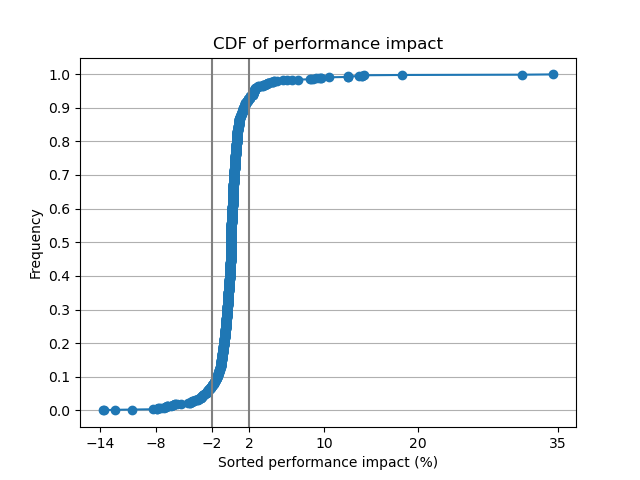
\includegraphics{perf-cdf}

%%% References

%% Note: use of BibTeX als works!!
\end{multicols}

\end{document}
